
% part 9
%A Second Interlude, Deferred
\section{Deferred'ы, часть вторая\label{sec:part9}}

%More Consequence of Callbacks
\subsection{Дальнейшие выводы про callback'и}

%We’re going to pause for a moment to think about callbacks again. Although we now know enough about deferreds to write simple asynchronous programs in the Twisted style, the Deferred class provides more features that only come into play in more complex settings. So we’re going to think up some more complex settings and see what sort of challenges they pose when programming with callbacks. Then we’ll investigate how deferreds address those challenges.
Мы ненадолго приостановимся, чтобы снова подумать о callback'ах. 
Хотя сейчас мы достаточно знаем о deferred'ах, для того, чтобы 
писать асинхронные программы в стиле Twisted, класс Deferred 
предоставляет больше свойств, которые имеют значение в более 
сложных настройках. Поэтому мы придумаем более сложные настройки и 
посмотрим какие преимущества мы получаем при программировании 
с использованием callback'ов. Затем мы изучим то, как deferred'ы 
используют эти преимущества.   


%To motivate our discussion we’re going to add a hypothetical feature to our poetry client. Suppose some hard-working Computer Science professor has invented a new poetry-related algorithm, the Byronification Engine. This nifty algorithm takes a single poem as input and produces a new poem like the original, but written in the style of Lord Byron. What’s more, our professor has kindly provided a reference implementation in Python, with this interface:

Для мотивации нашей дискуссии, добавим гипотетическое возможность 
к нашему поэтическому клиенту. Допустим, что некий профессор изобрел 
новый алгоритм, имеющий отношение к поэзии: Byronification Engine. 
Ловкий алгоритм берет на вход одну поэму и производит новую поэму, 
подобную первоначальной, но написанной в стиле 
\href{http://en.wikipedia.org/wiki/George\_Gordon\_Byron,\_6th\_Baron\_Byron}{Лорда Байрона}. 
Помимо этого, наш профессор любезно предоставляет ссылку на 
реализацию на Python'е со следующим интерфейсом:


\begin{scriptsize}\begin{verbatim}
class IByronificationEngine(Interface):

    def byronificate(poem):
        """
        Return a new poem like the original, but in the style of Lord Byron.

        Raises GibberishError if the input is not a genuine poem.
        """
\end{verbatim}\end{scriptsize}


%Like most bleeding-edge software, the implementation has some bugs. This means that in addition to the documented exception, the byronificate method sometimes throws random exceptions when it hits a corner-case the professor forgot to handle.
Подобно большиству передовых программ, реализация 
имеет какие-то баги. Это означает, что в дополнение к 
документированным исключениям, метод byronificate иногда 
выкидывает произвольные исключения, когда натыкается на 
случаи, которые профессор забыл отловить.


%We’ll also assume the engine runs fast enough that we can just call it in the main thread without worrying about tying up the reactor. This is how we want our program to work:
Мы будем также предполагать, что движок выполняется достаточно 
быстро, поэтому мы можем просто его вызывать из основного треда, 
не беспокоясь о связывании с реактором. Вот как хочется, чтобы 
работала программа:

\begin{enumerate}

%   1. Try to download the poem.
\item Попробовать скачать поэму.

%   2. If the download fails, tell the user we couldn’t get the poem.
\item Если скачивание не произошло из-за ошибки, сказать пользователю, 
что мы не можем получить поэму.

%   3. If we do get the poem, transform it with the Byronification Engine.
\item Если мы получили поэму, преобразовать ее с помощью движка Byronification.

%   4. If the engine throws a GibberishError, tell the user we couldn’t get the poem.
\item Если движок выкинул исключение GibberishError, сказать 
пользователю, что мы не можем получить поэму.

%   5. If the engine throws another exception, just keep the original poem.
\item Если движок выкинул какое-то другое исключение, 
сохранить первоначальную поэму.

%   6. If we have a poem, print it out.
\item Если мы имеем поэму - распечать ее.

%   7. End the program.
\item Завершить программу.

\end{enumerate}

%The idea here is that a GibberishError means we didn’t get an actual poem after all, so we’ll just tell the user the download failed. That’s not so useful for debugging, but our users just want to know whether we got a poem or not. On the other hand, if the engine fails for some other reason then we’ll use the poem we got from the server. After all, some poetry is better than none at all, even if it’s not in the trademark Byron style.
Здесь идея в том, что GibberishError означает, что в конце концов 
мы не получили действительную поэму, поэтому мы просто скажем 
пользователю, что скачивание завершилось с ошибкой. Это не особо 
полезно при отладке, но наши пользователи просто хотят 
знать: мы получили поэму или нет. С другой стороны, если движок 
завершается с ошибкой по какой-то причине, то мы будем использовать 
поэму, которую мы получили из сервера. В конце концов, какая-нибудь 
поэзия лучше, чем никакой, даже если она не под торговой маркой "стиль Байрона". 


%Here’s the synchronous version of our code:
Далее синхронная версия нашего кода:


\begin{scriptsize}\begin{verbatim}
try:
    poem = get_poetry(host, port) # synchronous get_poetry
except:
    print >>sys.stderr, 'The poem download failed.'
else:
    try:
        poem = engine.byronificate(poem)
    except GibberishError:
        print >>sys.stderr, 'The poem download failed.'
    except:
        print poem # handle other exceptions by using the original poem
    else:
        print poem

sys.exit()
\end{verbatim}\end{scriptsize}


%This sketch of a program could be make simpler with some refactoring, but it illustrates the flow of logic pretty clearly. We want to update our most recent poetry client (which uses deferreds) to implement this same scheme. But we won’t do that until Part 10. For now, instead, let’s imagine how we might do this with client 3.1, our last client that didn’t use deferreds at all. Suppose we didn’t bother handling exceptions, but instead just changed the got_poem callback like this:

Это набросок программы мог бы быть проще с некоторыми улучшениями, но он 
достаточно ясно иллюстрирует логический поток. Мы хотим обновить наш 
последний поэтический клиент (который использует deferred'ы), чтобы 
реализовать эту же схему. Но мы не будем делать до следующей главы. 
Сейчас, вместо этого, давайте представим то, как мы могли бы сделать 
это с  
\href{http://github.com/jdavisp3/twisted-intro/blob/master/twisted-client-3/get-poetry-1.py}{клиентом 3.1},  
нашим последний клиентом, который не использует deferred'ы. Предположим. что мы 
не заботимся управлением исключениями, но вместо этого мы меняем 
\href{http://github.com/jdavisp3/twisted-intro/blob/master/twisted-client-3/get-poetry-1.py#L106}{got\_poem} 
callback следующим образом:


\begin{scriptsize}\begin{verbatim}
def got_poem(poem):
    poems.append(byron_engine.byronificate(poem))
    poem_done()
\end{verbatim}\end{scriptsize}


%What happens when the byronificate method raises a GibberishError or some other exception? Looking at Figure 11 from Part 6, we can see that:
Что происходит, когда метод byronificate генерирует GibberishError или 
какое-то другое исключение? Смотря на рисунок \ref{fig:reactor-poem-callback}, 
мы можем увидеть что: 

\begin{enumerate}
   
%   1. The exception will propagate to the poem_finished callback in the factory, the method that actually invokes the callback.
\item Исключение будет передаваться к callback'у poem\_finished в factory, 
методу, который в действительности вызывает callback. 

%   2. Since poem_finished doesn’t catch the exception, it will proceed to poemReceived on the protocol.
\item Поскольку poem\_finished не ловит исключения, далее продолжится 
выполнение в методе poemReceived протокола. 

%   3. And then on to connectionLost, also on the protocol.
\item Затем в connectionLost также протокола.

%   4. And then up into the core of Twisted itself, finally ending up at the reactor.
\item Затем управление перейдет самому Twised, окончательно 
завершись в реакторе. 

\end{enumerate}

%As we have learned, the reactor will catch and log the exception instead of crashing. But what it certainly won’t do is tell the user we couldn’t download a poem. The reactor doesn’t know anything about poems or GibberishErrors, it’s a general-purpose piece of code used for all kinds of networking, even non-poetry-related networking.
Как мы изучили, reactor ловит и логирует 
исключения, а не завершается с ошибкой. Но то, что он 
определенно не сделает - не скажет пользователю, что 
мы не смогли скачать поэму. reactor ничего не знает о поэмах 
или об исключениях типа GibberishError, это код общего 
назначения для всех видов сетевых взаимодейтсвий, даже 
не относящихся к поэзии.


%Notice how, at each step in the list above, the exception moves to a more general-purpose piece of code than the one before. And at no step after got_poem is the exception in a piece of code that could be expected to handle an error in the specific way we want for this client. This situation is basically the exact opposite of the way exceptions propagate in synchronous code.
Заметьте, как на каждом шаге в списке выше, 
исключение перемещается к коду, имеющему более и более  
общее назначение. В got\_poem нет кода специфичного для нашего 
клиента управления исключениями. Эта ситуация противоположна тому, как
исключения распостраняются в синхронном коде.


%Take a look at Figure 15, an illustration of a call stack we might see with a synchronous poetry client :
Давайте посмотрим на рисунок \ref{fig:sync-exceptions}, 
иллюстрацию стека вызова, которую мы можем увидеть в 
синхронном поэтическом клиенте:

% fig15
\begin{figure}[h]
\begin{center}
    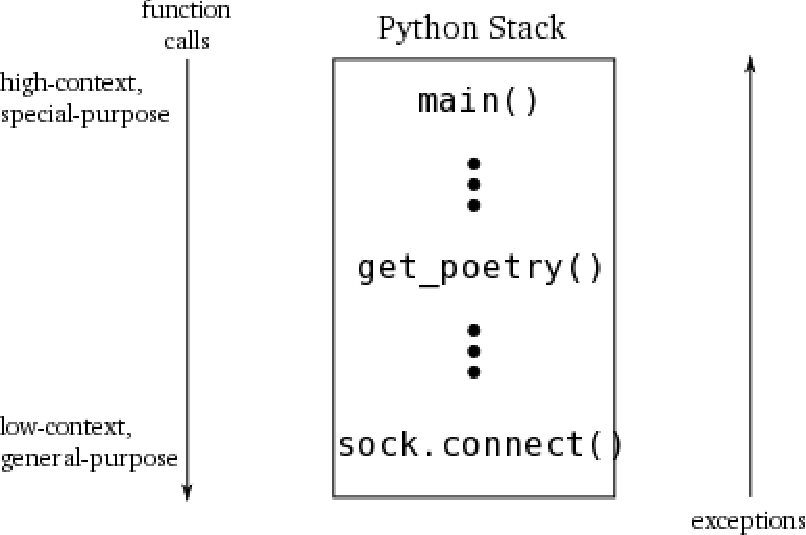
\includegraphics[width=0.4\textwidth]{images/sync-exceptions.pdf}
    \caption{Cинхронный код и исключения\label{fig:sync-exceptions}}
\end{center}
\end{figure}


%The main function is “high-context”, meaning it knows a lot about the whole program, why it exists, and how it’s supposed to behave overall. Typically, main would have access to the command-line options that indicate just how the user wants the program to work (and perhaps what to do if something goes wrong). It also has a very specific purpose: running the show for a command-line poetry client.
Функция main - это "высокоуровневая", что означает, что она 
много знает о всей программе, почему она выходит, предполагаемое 
поведение в целом. Типично, main имела бы доступ к опциям командной 
строки, которая означает то, как пользователь хочет, чтобы 
программа работала (и, возможно, что надо делать, если что-то 
пошло не так).
 

%The socket connect method, on the other hand, is “low-context”. All it knows is that it’s supposed to connect to some network address. It doesn’t know what’s on the other end or why we need to connect right now. But connect is quite general-purpose — you can use it no matter what sort of service you are connecting to.
С другой стороны, метод connect модуля socket, "низкоуровневый". 
Все что он знает - это то, что предполагается присоединиться по 
некоторому сетевому адресу. Он даже не знает, что на другом конце, или 
почему нам нужно соединиться прямо сейчас. Но connect - метод общего 
назначения, вы можете его использовать, невзирая на тип сервиса, к 
которому вы присоединяетесь.


%And get_poetry is in the middle. It knows it’s getting some poetry (and that’s the only thing it’s really good at), but not what should happen if it can’t.
А метод get\_poetry находится по середине. Он знает, что он получает 
некоторую поэзию (и это единственное, чем он занимается), но не знает, 
что должно произойти, если он не сможет получить поэзию.
 

%So an exception thrown by connect will  move up the stack, from low-context and general-purpose code to high-context and special-purpose code, until it reaches some code with enough context to know what to do when something goes wrong (or it hits the Python interpreter and the program crashes).
Таким образом, исключение, произошеднее в connect'е, будет 
перемещаться вверх по стеку, из низкоуровнего контекста и 
кода общего назначения в высокоуровневый контекст и кода 
специального назначения до тех пор, пока он не достигнет 
некоторого кода с контекстом, который будет знать, что делать, 
когда что-то пошло не так (или оно поймается интерпретатором 
Python'а и программа развалится).
 

%Of course the exception is really just moving up the stack no matter what rather than literally seeking out high-context code. It’s just that in a typical synchronous program “up the stack” and “towards higher-context” are the same direction.
Конечно же, исключение в действительности просто перемещается вверх 
по стеку, не разыскивая, что является более "высококонтекстным кодом". 
Это потому что в типичной синхронной программе "ввер по стеку" и 
"в направлении высокоуровневого контекста" - это одно и то же.

\eject

%Now recall our hypothetical modification to client 3.1 above. The call stack we analyzed is pictured in Figure 16, abbreviated to just a few functions:
Теперь вспомним гипотетическую модификацию клиента 3.1 выше. 
Стек вызова, который мы анализировали, изображен на рисунке \ref{fig:async-exceptions}, 
сокращенный только до нескольких функций:

% fig16
\begin{figure}[h]
\begin{center}
    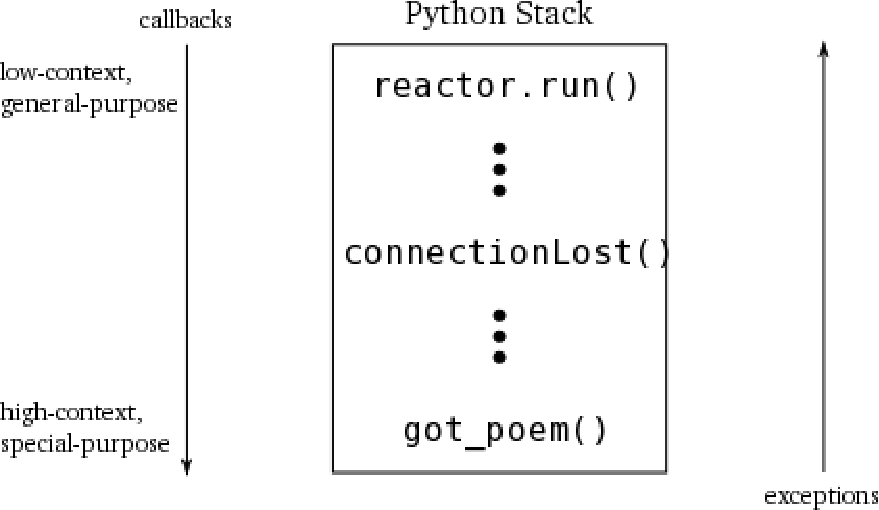
\includegraphics[width=0.4\textwidth]{images/async-exceptions.pdf}
    \caption{Асинхронные callback'и и исключения\label{fig:async-exceptions}}
\end{center}
\end{figure}

%The problem is now clear: during a callback, low-context code (the reactor) is calling higher-context code which may in turn call even higher-context code, and so on. So if an exception occurs and it isn’t handled immediately, close to the same stack frame where it occurred, it’s unlikely to be handled at all. Because each time the exception moves up the stack it moves to a piece of lower-context code that’s even less likely to know what to do.
Проблема теперь ясна: во время callback'а, низкоуровневый код (reactor) 
вызывает высокоуровневый код, который в свою очередь может вызвать более 
высокоуровневый код и так далее. Таким образом, если происходит исключение, и 
оно немедленно не обрабатывается примерно в том же stack frame'е, где оно 
произошло, то оно, вероятно, не будет обработано вовсе. Поскольку каждый раз, 
когда исключение перемещается вверх по стеку, оно перемещается к низкоуровневому 
коду, который еще менее вероятно знает, что делать.


%Once an exception crosses over into the Twisted core the game is up. The exception will not be handled, it will only be noted (when the reactor finally catches it). So when we are programming with “plain old” callbacks (without using deferreds), we must be careful to catch every exception before it gets back into Twisted proper, at least if we want to have any chance of handling errors according to our own rules. And that includes exceptions caused by our own bugs!
Как только исключение перейдет в Twisted код, то все пропало. 
Исключение не будет обработано, оно будет только замечено (когда reactor 
окончательно его поймает). Поэтому, когда мы программируем с обычными 
callback'ми (без использования deferred'ов), мы должны тщательно 
отлавливать каждое исключение до того, как оно вовзвратится в 
Twisted, по меньшей мере, если мы хотим иметь какой-то шанс управления 
ошибками согласно нашим правилам. Это также касается ошибок, вызванных  
нашими багами!


%Since a bug can exist anywhere in our code, we would need to wrap every callback we write in an extra “outer layer” of try/except statements so the exceptions from our fumble-fingered typos can be handled as well. And the same goes for our errbacks because code to handle errors can have bugs too.
Поскольку баг может присутствовать в любом месте нашего кода, нам нужно было 
бы оборачивать каждый callback, который мы пишем, в дополнительный уровень 
из операторов try/except так, чтобы исключения из наших нелепостей, могли 
быть обработаны.  Тоже самое касается наших errback'ов, поскольку код для 
управления ошибками, может также иметь баги. 


%Well that’s not so nice.
И это не особо хорошо.


%The Fine Structure of Deferreds
\subsection{Прекрасная структура Deferred'ов}

%It turns out the Deferred class helps us solve this problem. Whenever a deferred invokes a callback or errback, it catches any exception that might be raised. In other words, a deferred acts as the “outer layer” of try/except statements so we don’t need to write that layer after all, as long as we use deferreds. But what does a deferred do with an exception it catches? Simple — it passes the exception (in the form of a Failure) to the next errback in the chain.
Оказывается, класс Deferred помогает решить нам эту проблему. 
В момент, когда deferred вызывает callback и errback, он 
ловит любое исключение, которое могло бы произойти. Другими 
словами, deferred действует как "внешний уровень" из операторов 
try/except, так что, в конце концов, нам не нужно писать этот уровень, 
в случае использования deferred'ов. Но что делает deferred 
с исключением, которые он ловит? Все просто: он подставляет исключение (в виде Failure) 
следующему errback'у в цепочке.


%So the first errback we add to a deferred is there to handle whatever error condition is signaled when the deferred’s .errback(err) method is called. But the second errback will handle any exception raised by either the first callback or the first errback, and so on down the line.
Так как первый errback, который мы добавляем в deferred, 
является тем местом, где обрабатывается какое-нибудь 
условие ошибки, которое сигнализируется вызовом метода 
deferred'а errback. Второй errback будет обрабатывать исключение, 
возникшее или в первом callback'е, или в первом 
errback'e, и так далее вниз по цепочке.


%Recall Figure 12, a visual representation of a deferred with some callbacks and errbacks in the chain. Let’s call the first callback/errback pair stage 0, the next pair stage 1, and so on.
Вспомним \ref{fig:deferred-1}, визуальное представление deferred'а с 
некоторыми callback'ми и errback'ми в цепочке. Давайте назовем первую 
пару callback/errback этапом 0, следующую - 1 и т.д.


%At a given stage N, if either the callback or the errback (whichever was executed) fails, then the errback in stage N+1 is called with the appropriate Failure object and the callback in stage N+1 is not called.
В заданной стадии N, если callback или errback (какой бы ни выполнялся) 
завершаются с ошибкой, то будет вызван errback из этапа N+1 с 
соответсвующим объектом типа Failure, и callback из этапа N+1 
не будет вызван. 


%By passing exceptions raised by callbacks “down the chain”, a deferred moves exceptions in the direction of “higher context”. This also means that invoking the callback and errback methods of a deferred will never result in an exception for the caller (as long as you only fire the deferred once!), so lower-level code can safely fire a deferred without worrying about catching exceptions. Instead, higher-level code catches the exception by adding errbacks to the deferred (with addErrback, etc.).
Подставляя исключения, сгерерированных callback'ми, 
"вниз по цепочке", deferred перемещает исключения в 
направлеии "высокоуровневого контекста". Это также 
означает, что вызывающиеся методы deferred'а callback и errback 
никогда не сгенерируют исключение тому, кто их вызвал (конечно, 
если вы активизируете deferred только один раз!), поэтому 
низкоуровневый код может безопасно активизировать deferred, 
не заботясь об отлавливании исключений. В то время как, 
высокоуровневый код поймает исключения, добавляя 
errback'и в deferred (с помощью, например, addErrback).


%Now in synchronous code, an exception stops propagating as soon as it is caught. So how does an errback signal the fact that it “caught” the error? Also simple — by not raising an exception. And in that case, the execution switches over to the callback line. So at a given stage N, if either the callback or errback succeeds (i.e., doesn’t raise an exception) then the callback in stage N+1 is called with the return value from stage N, and the errback in stage N+1 is not called.
В синхронном коде, исключения прекращают 
распостраняться после их первого отлавливания. 
А как же errback сигнализирует о том, что он "поймал" ошибку? 
Также просто: не генерируя исключение. В этом 
случае, выполнение переключится на callback-цепочку. Так что 
если на заданном этапе N, либо callback, либо errback завершаются 
успешно (например, не генерируют исключение), то вызывается
callback из этапа N+1 со значением, возвращенным из этапа N, и 
errback из этапа N+1 не вызывается.  


%Let’s summarize what we know about the deferred firing pattern:
Давайте подведем итоги того, что мы знаем об активизации deferred'а:

\begin{enumerate}

%   1. A deferred contains a chain of ordered callback/errback pairs (stages). The pairs are in the order they were added to the deferred.
\item deferred содержит цепочку упорядоченных пар callback/errback (этапов). 
Пары находятся в порядке, в котором они добавлялись в deferred.

%   2. Stage 0, the first callback/errback pair, is invoked when the deferred is fired. If the deferred is fired with the callback method, then the stage 0 callback is called. If the deferred is fired with the errback method, then the stage 0 errback is called.
\item Этап 0, первая пара callback/errback, вызывается, когда 
активизируется deferred. Если deferred активизируется с методом 
callback, то вызывается callback из этапа 0. Если deferred 
активизируется методом errback, то вызывается errback из этапа 0. 

%   3. If stage N fails, then the stage N+1 errback is called with the exception (wrapped in a Failure) as the first argument.
\item Если на этапе N происходит ошибка, то 
вызывается errback из этапа N+1 с исключением (обернутым в Failure) в 
качестве первого аргумента.

%   4. If stage N succeeds, then the stage N+1 callback is called with the stage N return value as the first argument.
\item Если этап N успешно завершается, то вызывается callback из 
этапа N+1 со значением, возвращенным этапом N+1, в качестве первого аргумента.

\end{enumerate}


%This pattern is illustrated in Figure 17:
Этот шаблон проиллюстрирован на рисунке \ref{fig:deferred-2}:

% fig17
\begin{figure}[h]
\begin{center}
    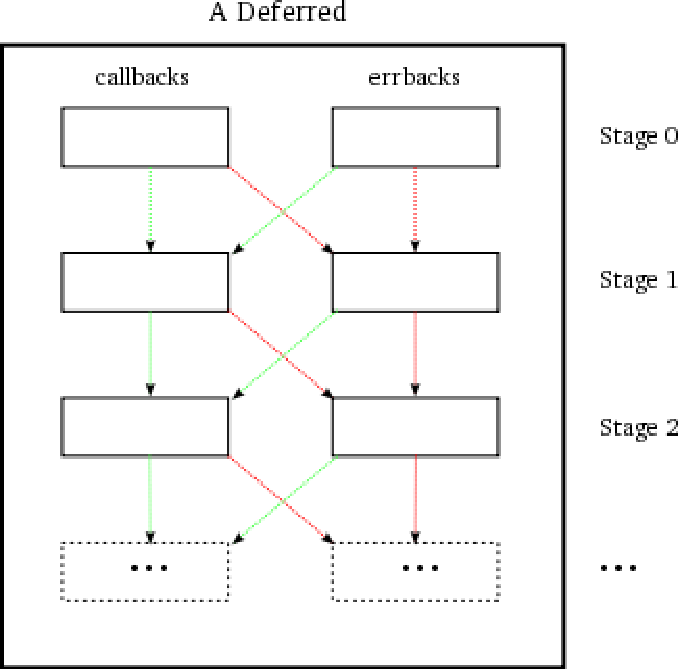
\includegraphics[height=0.3\textheight]{images/deferred-2.pdf}
    \caption{Поток управления в deferred'е\label{fig:deferred-2}}
\end{center}
\end{figure}


%The green lines indicate what happens when a callback or errback succeeds and the red lines are for failures. The lines show both the flow of control and the flow of exceptions and return values down the chain. Figure 17 shows all possible paths a deferred might take, but only one path will be taken in any particular case. Figure 18 shows one possible path for a “firing”:
Зеленые линии показывают, что происходит, когда 
callback или errback успешно завершаются, и 
красные линии, если завершаются с ошибками. 
Линии показывают оба поток управления и исключений и 
возвращаемые значения вниз по цепочке. Рисунок \ref{fig:deferred-2} 
показывает все возможные пути, которыми deferred 
может быть пройти, но только один путь возьмется из определенного 
случая. Рисунок \ref{fig:deferred-3} показывает один 
возможный путь для "активизации": 

% fig18
\begin{figure}[h]
\begin{center}
    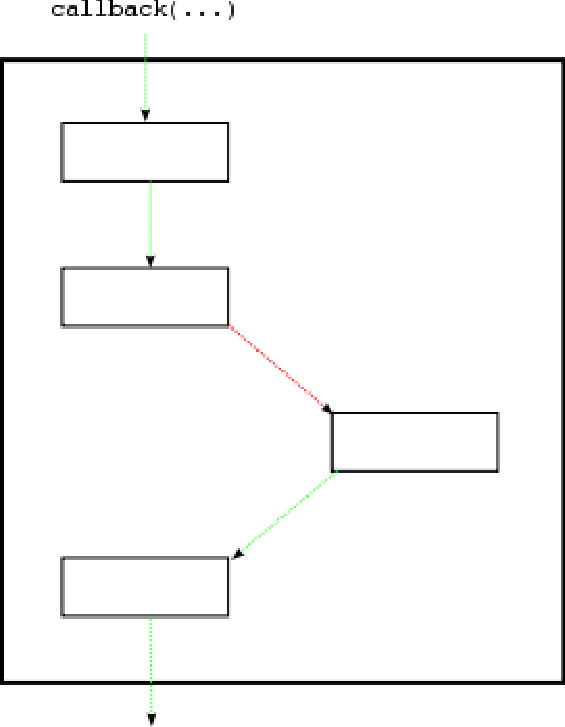
\includegraphics[height=0.3\textheight]{images/deferred-3.pdf}
    \caption{Один из возможных способов активизации deferred'а\label{fig:deferred-3}}
\end{center}
\end{figure}


%In figure 18, the deferred’s callback method is called, which invokes the callback in stage 0. That callback succeeds, so control (and the return value from stage 0) passes to the stage 1 callback. But that callback fails (raises an exception), so control switches to the errback in stage 2. The errback “handles” the error (it doesn’t raise an exception) so control moves back to the callback chain and the callback in stage 3 is called with the result from the stage 2 errback.
На рисунке \ref{fig:deferred-3} вызывается метод callback deferred'а, 
который вызывает callback из этапа 0. Этот callback успешно завершается, 
поэтому управление (и возвращаемое значение из этапа 0) передается 
callback'у из этапа 1. Но callback из этапа 1 завершается с ошибкой (генерирует 
исключение), поэтому управление переключается на errback из этапа 2. errback 
"обрабатывает" ошибку (не генерирует исключение), поэтому контроль 
переходит обратно к callback'у из этапа 3.


%Notice that any path you can make with Figure 17 will pass through every stage in the chain, but only one member of the callback/errback pair at any stage will be called.
Заметьте, что любой путь из рисунка \ref{fig:deferred-2} будет 
проходить через каждый этап цепочки, но только один из пары 
callback/errback для каждой стадии будет вызван.
 

%In Figure 18, we’ve indicated that the stage 3 callback succeeds by drawing a green arrow out of it, but since there aren’t any more stages in that deferred, the result of stage 3 doesn’t really go anywhere. If the callback succeeds, that’s not really a problem, but what if it had failed? If the last stage in a deferred fails, then we say the failure is unhandled, since there is no errback to “catch” it.
На рисунке \ref{fig:deferred-3}, мы показали, что на этапе 3 
callback успешно завершается, нарисовав выходящую зеленую стрелку, 
но поскольку нет больше этапов в deferred'е, то результат этапа 3 
никуда в действительности не отправится. Если callback завершается 
успешно, то это в действительности не проблема, но что, если 
callback завершился с ошибкой? Если последний этап в deferred'е 
завершился с ошибкой, то мы говорим, что ошибка не обработывается, 
поскольку нет errback'а, который ее "поймает".


%In synchronous code an unhandled exception will crash the interpreter, and in plain-old-callbacks asynchronous code an unhandled exception is caught by the reactor and logged. What happens to unhandled exceptions in deferreds? Let’s try it out and see. Look at the sample code in twisted-deferred/defer-unhandled.py. That code is firing a deferred with a single callback that always raises an exception. Here’s the output of the program:
В синхронном коде необработанные исключения рушат 
интерпретатор, и необработанные исключение в обычных callback'ах 
асинхронного кода ловятся реактором и логируются. Что 
происходит с необработанными исключениями в deferred'ах? 
Давайте попробуем так сделать и посмотрим. Посмотрите на 
пример в 
\href{http://github.com/jdavisp3/twisted-intro/blob/master/twisted-deferred/defer-unhandled.py#L1}{twisted-deferred/defer-unhandled.py}. 
Этот код активизирует deferred с одним callback'ом, который 
всегда генерирует исключение. Далее вывод программы:


\begin{scriptsize}\begin{verbatim}
Finished
Unhandled error in Deferred:
Traceback (most recent call last):
  ...
--- <exception caught here> ---
  ...
exceptions.Exception: oops
\end{verbatim}\end{scriptsize}



%Some things to notice:
Надо отметить следующее:

\begin{enumerate}

%   1. The last print statement runs, so the program is not “crashed” by the exception.
\item Последний оператор print выполняется, так что программа не 
рушится исключением.

%   2. That means the Traceback is just getting printed out, it’s not crashing the interpreter.
\item Это означает, что traceback просто печатается, и это не разрушенный интерпретатор.

%   3. The text of the traceback tells us where the deferred itself caught the exception.
\item Текст traceback'а говорит нам, где deferred сам поймал исключение.

%   4. The “Unhandled” message gets printed out after “Finished”.
\item Сообщение "Unhandled" печатается после "Finished".

\end{enumerate}


%So when you use deferreds, unhandled exceptions in callbacks will still be noted, for debugging purposes, but as usual they won’t crash the program (in fact they won’t even make it to the reactor, the deferred will catch them first). By the way, the reason that “Finished” comes first is because the “Unhandled” message isn’t actually printed until the deferred is garbage collected. We’ll see the reason for that in a future Part.
Поэтому, когда мы используем deferred'ы, необработанные 
исключения в callback'ах все еще будут замечены для 
целей отладки, но они не будут рушить программу (фактически, 
они не будут передаваться реактору, deferred'ы первыми их поймают). 
Кстати, причина почему "Finish" печатается первым связана с тем, 
что сообщение "Unhandled" в действительности не печаетается 
до тех пор, пока deferred  не утилизируется сборщиком мусора. 
Мы увидим причину в следующей главе.


%Now, in synchronous code we can “re-raise” an exception using the raise keyword without any arguments. Doing so raises the original exception we were handling and allows us to take some action on an error without completely handling it. It turns out we can do the same thing in an errback. A deferred will consider a callback/errback to have failed if:
В синхронном коде мы можем "перевызвать" исключение, 
используя ключевое слово raise без аргументов. Делая так, 
мы вызываем первоначальное исключение, которое мы обрабатывали, 
что позволяет нам произвести какие дополнительные действия без 
полной его обработки. В свою очередь, мы может сделать тоже 
самое с errback'ом. deferred будет считать, что 
callback/errback завершился с ошибкой, если:  

\begin{itemize}

%    * The callback/errback raises any kind of exception, or
\item callback/errback вызывает любой тип исключения, или

%    * The callback/errback returns a Failure object.
\item callback/errback возвращает объект типа Failure.

\end{itemize}


%Since an errback’s first argument is always a Failure, an errback can “re-raise” the exception by returning its first argument, after performing whatever action it wants to take.
Поскольку первый аргумент errback'а всегда типа Failure, 
errback может "перевызвать" исключение, возвратив 
свой первый аргумент, после выполнения какого-либо 
действия.


%Callbacks and Errbacks, Two by Two
\subsection{Callback'и и Errback'и, по двое}

%One thing that should be clear from the above discussion is that the order you add callbacks and errbacks to a deferred makes a big difference in how the deferred will fire. What should also be clear is that, in a deferred, callbacks and errbacks always occur in pairs. There are four methods on the Deferred class you can use to add pairs to the chain:
Одно должно быть ясно из обсуждения выше - это то, что 
порядок, в котором вы добавляете callback'и и errback'и в 
deferred, определяет порядок, в котором они будут активизированы. 
Что еще должно быть ясно - это то, что в deferred'е callback'и и 
errback'и всегда появляются парами. Есть 4 метода в классе 
Deffered, которые вы можете использовать для добавления пар 
в цепочку:

\begin{enumerate}
\item addCallbacks
\item addCallback
\item addErrback
\item addBoth
\end{enumerate}


%Obviously, the first and last methods add a pair to the chain. But the middle two methods also add a callback/errback pair. The addCallback method adds an explicit callback (the one you pass to the method) and an implicit “pass-through” errback. A pass-through function is a dummy function that just returns its first argument. Since the first argument to an errback is always a Failure, a pass-through errback will always “fail” and send its error to the next errback in the chain.
Очевидно, что первый и последний методы добавляют 
пару в цепочку. Но два других метода также добавляют 
пару callback/errback. Метод addCallback добавляет явный 
callback (тот, который вы передали в метод) и неявный 
"сквозной" errback. Сквозная функция - это функция-заглушка, 
которая просто возвращает свой первый аргумент. Поскольку 
первый аргумент в errback'е всегда типа Failure, сквозной 
errback всгда завершается с ошибкой и отправляет ошибку 
следующему errback'у в цепочке.


%As you’ve no doubt guessed, the addErrback function adds an explicit errback and an implicit pass-through callback. And since the first argument to a callback is never a Failure, a pass-through callback sends its result to the next callback in the chain.
Как вы несомненно догадались, функция addErrback добавляет 
явный errback и неявный сквозной callback. И поскольку первый 
аргумент в callback'е никогда не является Failure, 
сквозной callback отправляет свой результат следующему 
callback'у в цепочке.


%The Deferred Simulator
\subsection{Deferred симулятор}

%It’s a good idea to become familiar with the way deferreds fire their callbacks and errbacks. The python script in twisted-deferred/deferred-simulator.py is a “deferred simulator”, a little python program that lets you explore how deferreds fire. When you run the script it will ask you to enter list of callback and errback pairs, one per line. For each callback or errback, you specify that either:
Хорошая идея познакомиться о том, как deferred'ы 
активизируют свои callback'и и errback'и. В 
\href{http://github.com/jdavisp3/twisted-intro/blob/master/twisted-deferred/deferred-simulator.py#L1}{twisted-deferred/deferred-simulator.py} 
находится python скрипт, являющийся "deferred симулятором", 
небольшая программа, которая позволяет вам 
раскрыть то, как deferred'ы активизируют свои цепочки. 
Когда вы запустите скрипт, он попросит вам ввести список пар 
callback/errback в одну строку. Для каждого callback'а или 
errback'а вы задаете одно из:

\begin{itemize}

%    * It returns a given value (succeds), or
\item Он возвращает заданное значение (выполнение без ошибок)

%    * It raises a given exception (fails), or
\item Он вызывает данное исключение (выполнение с ошибкой)

%    * It returns its argument (passthru).
\item Он возвращает свой аргумент (сквозное выполнение)

\end{itemize}


%After you’ve entered all the pairs you want to simulate, the script will print out, in high-resolution ASCII art, a diagram showing the contents of the chain and the firing patterns for the callback and errback methods. You will want to use a terminal window that is as wide as possible to see everything correctly. You can also use the --narrow option to print the diagrams one after the other, but it’s easier to see their relationships when you print them side-by-side.
После того, как вы ввели все пары, и вы хотите 
симулировать, скрипт напечатает диаграмму, показывающую 
содержимое цепочки и шаблоны активизации для методов 
callback и errback. Вы можете использовать терминальное 
окно, которое настолько широко, насколько это возможно, 
для того, чтобы увидеть все корректно. Вы также можете 
использовать опцию --narrow для распечатки диаграмма 
одну за другой, но проще увидеть их взаимосвязь при их 
распечатке бок о бок. 


%Of course, in real code a callback isn’t going to return the same value every time, and a given function might sometimes succeed and other times fail. But the simulator can give you a picture of what will happen for a given combination of normal results and failures, in a given arrangement of callbacks and errbacks.
Конечно же, в реальном коде callback не будет 
возвращать одно и тоже значение каждый раз, и 
данная функция может иногда завершиться успешно, 
иногда - с ошибкой. Но симулятор может дать 
представление того, что произойдет для 
заданной комбинации результатов и ошибок, в заданной 
композиции callback'ов и errback'ов.


\subsection{Резюме}

%After thinking some more about callbacks, we realize that letting callback exceptions bubble up the stack isn’t going to work out so well, since callback programming inverts the usual relationship between low-context and high-context code. And the Deferred class tackles this problem by catching exceptions and sending them down the chain instead of up into the reactor.
Немного больше подумав о callback'ах, мы осознали, что 
позволяя callback исключениям всплывать вверх по стеку, 
не приведет ни к чему хорошему, поскольку программирование 
с использованием callback'ов инвертирует обычную взаимосвязь 
между низкоуровневым и высокоуровневым кодом. Класс Deferred 
решает эту проблему, отлавливая исключения и отправляя из вниз по 
цепочке, вместо вверх, в reactor.
 

%We’ve also learned that ordinary results (return values) move down the chain as well. Combining both facts together results in a kind of criss-cross firing pattern as the deferred switches back and forth between the callback and errback lines, depending on the result of each stage.
Мы также изучили, что обычные результаты (возвращаемые значение) 
также перемещаются вниз по цепочке. Комбинирую оба факта вместе, дают 
в результате шаблон активизации крест-накрест, так как deferred 
переключается между callback и errback цепочками, взависимости от 
результата на каждом этапе.


%Armed with this knowledge, in Part 10 we will update our poetry client with some poetry transformation logic.
Вооружившись эти знанием, в следующей главе мы 
обновим наш поэтический клиент с некоторой поэтической 
трансформирующей логикой.


\subsection{Упражнения}

\begin{enumerate}

%   1. Inspect the implementation of each of the four methods on the Deferred which add callbacks and errbacks. Verify that all methods add a callback/errback pair.
\item Изучите реализацию каждого из четырех методов в классе 
\href{http://twistedmatrix.com/trac/browser/tags/releases/twisted-8.2.0/twisted/internet/defer.py#L172}{Deferred}, 
 
которые добавляют callback'и и errback'и. Проверьте, что все методы 
добавляют пару callback/errback. 

%   2. Use the deferred simulator to investigate the difference between this code:
\item Используйте deferred симулятор для того, чтобы изучить отличие между этим кодом:


\begin{scriptsize}\begin{verbatim}
      deferred.addCallbacks(my_callback, my_errback)
\end{verbatim}\end{scriptsize}


%      and this code:
и этим кодом:


\begin{scriptsize}\begin{verbatim}
      deferred.addCallback(my_callback)
      deferred.addErrback(my_errback)
\end{verbatim}\end{scriptsize}


%      Recall that the last two methods add implicit pass-through functions as one member of the pair. 
Вспомните, что два последних метода добавляют неявные сквозные 
функции в качестве одного из членов пары.

\end{enumerate}

